\newpage
\section{Suddivisione del lavoro}
Nei seguenti paragrafi verrà spiegato come il gruppo intende dividere l'impegno dei ruoli nei sei diversi periodi di sviluppo del software. Successivamente verranno inserite le ore di investimento complessive nel gruppo. Verrà spiegato inoltre come il gruppo intende dividere soddisfare alcune regole del progetto:
\begin{itemize}
	\item Tutti i componenti devono ricoprire almeno una volta tutti i ruoli; 
	\item Un componente del gruppo può ricoprire più ruoli contemporaneamente, a patto che non entri in conflitto d'interesse (ad esempio, non può verificare il lavoro da lui svolto).
\end{itemize}

All'ultimo paragrafo è presente un riassunto con il totale del peso dei vari ruoli nell'intero progetto.

\subsection{Periodo di Analisi dei Requisiti}
Il primo periodo è l'\AdR. Esso non è rendicontabile ai fini di calcolo del preventivo, poichè non è da considerarsi a carico del \textit{Proponente}. Le ore totali sono suddivise come segue:

\begin{table}[H]
	\begin{center}
		\begin{tabular}{|c|c|c|c|c|c|c|c|}
			\hline
			\textbf{Nome} & \multicolumn{6}{c|}{\textbf{Ore per ruolo}} & \textbf{Ore totali} \\\cline{2-7}
			& \textbf{Resp} & \textbf{Amm} & \textbf{An} & \textbf{Proj} & \textbf{Prog} & \textbf{Ver} & \\
			\hline
			\MC			&		&		&	16	&		&		&	15	&	31	\\
			\hline
			\AN			&		&	3	&	6	&	 	&		&	22	& 	31	\\
			\hline
			\DAN		&		&	3	&	29	&		&		&		&	32	\\
			\hline
			\AS			&	20	&	 	&	12 	&		&	 	& 		&	32	\\
			\hline
			\NS 		&	18	&	3	&	11	&		&		& 		&	32	\\
			\hline
			\DS			& 		&	2	&	5	&		&		&	24	&	31	\\
			\hline
			\textbf{Totali per ruolo}	& 	38	&	11	&	79	&		&		&	61	&	189	\\
			\hline
		\end{tabular}
	\end{center}
	\caption{Ore per componente, \AdR}
\end{table}

\begin{figure}[H]
	\centering
	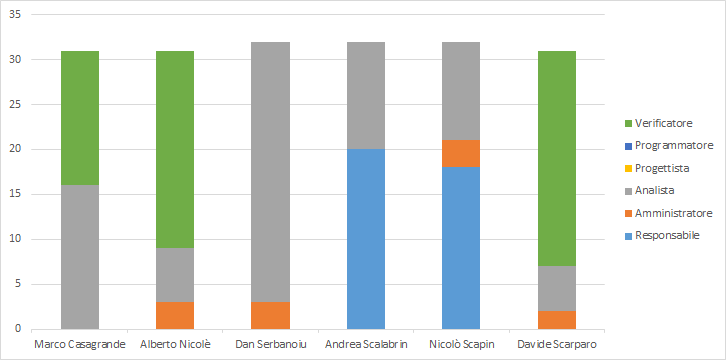
\includegraphics[scale=0.6]{img/6-1.png}
	\caption{Suddivisione ruoli per componente, Analisi dei Requisiti}
\end{figure}

L'incidenza di tali ore determina in percentuale, come mostrato di seguito:
\begin{figure}[H]
	\centering
	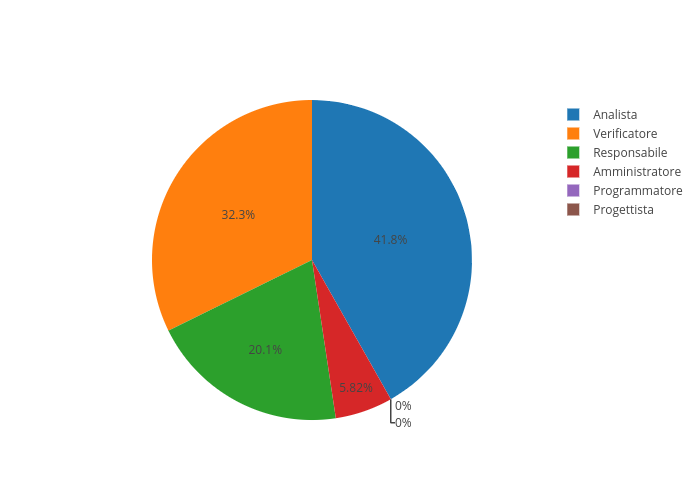
\includegraphics[scale=0.6]{img/AnalisiRequisiti.png}
	\caption{Incidenza ore per ruolo, periodo di Analisi dei Requisiti}
\end{figure}

\newpage
\subsection{Periodo di Analisi dei Requisiti Dettagliata}
La seconda porzione di \AdR, da svolgersi dopo la \RR, è l'Analisi dei Requisiti Dettagliata. Come per il precedente, esso è da considerarsi parte dell'investimento intrapreso e quindi, non è rendicontabile ai fini del calcolo del preventivo. 
Durante il periodo di \ARD, il lavoro dei membri sarà suddiviso come segue:

\begin{table}[H]
	\begin{center}
		\begin{tabular}{|c|c|c|c|c|c|c|c|}
			\hline
			\textbf{Nome} & \multicolumn{6}{c|}{\textbf{Ore per ruolo}} & \textbf{Ore totali} \\\cline{2-7}
			& \textbf{Resp} & \textbf{Amm} & \textbf{An} & \textbf{Proj} & \textbf{Prog} & \textbf{Ver} & \\
			\hline
			\MC			&		&	1	&	 	&		&		&	2 	&	 3	\\
			\hline
			\AN			&		&		&	3 	&	 	&		&	 	& 	 3	\\
			\hline
			\DAN		&		&	 	&	2 	&		&		&		&	 2	\\
			\hline
			\AS			&	2	&	 	&	  	&		&	 	& 		&	 2	\\
			\hline
			\NS 		&	2	&		&	 	&		&		& 		&	 2	\\
			\hline
			\DS			& 		&	 	&	 	&		&		&	3 	&	 3	\\
			\hline
			\textbf{Totali per ruolo}	& 	4	&	1	&	5	&		&		&	5	&	15	\\
			\hline
		\end{tabular}
	\end{center}
	\caption{Ore per componente, \ARD}
\end{table}

\begin{figure}[H]
	\centering
	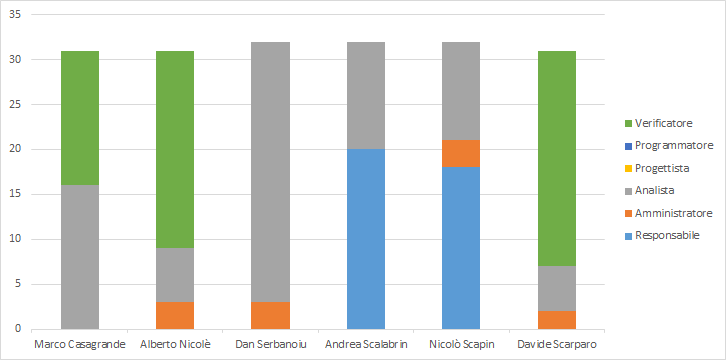
\includegraphics[scale=0.6]{img/6-1a.png}
	\caption{Suddivisione ruoli per componente, Analisi dei Requisiti Dettagliata}
\end{figure}

L'incidenza di tali ore determina in percentuale, come mostrato di seguito:
\begin{figure}[H]
	\centering
	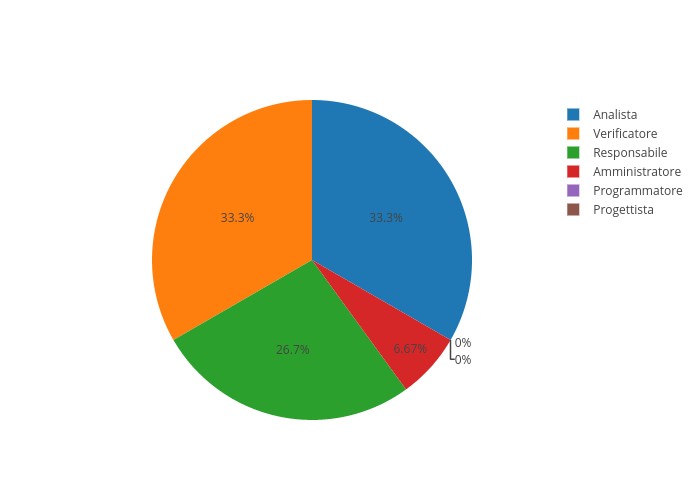
\includegraphics[scale=0.6]{img/AnalisiRequisitiDettaglio.png}
	\caption{Incidenza ore per ruolo, periodo di Analisi dei Requisiti Dettagliata}
\end{figure}

\newpage
\subsection{Periodo di Progettazione Architetturale}
Lo sviluppo procede con la Progettazione Architetturale. Durante il periodo di Progettazione Architetturale, il lavoro dei membri sarà suddiviso come segue:

\begin{table}[H]
	\begin{center}
		\begin{tabular}{|c|c|c|c|c|c|c|c|}
			\hline
			\textbf{Nome} & \multicolumn{6}{c|}{\textbf{Ore per ruolo}} & \textbf{Ore totali} \\\cline{2-7}
			& \textbf{Resp} & \textbf{Amm} & \textbf{An} & \textbf{Proj} & \textbf{Prog} & \textbf{Ver} & \\
			\hline
			\MC			&		&	3	&		&	31	&		&		&   34	\\
			\hline
			\AN			&	3	&		&		&	31	&		&		& 	34	\\
			\hline
			\DAN		&		&	2	&		&	17	&		&	14	&	33	\\
			\hline
			\AS			&		&	 	&	 	&	14	&	 	& 	19	&	33	\\
			\hline
			\NS 		&		&		&		&	14	&		& 	19	&	33	\\
			\hline
			\DS			& 	2	&		&		&	31	&		&		&	33	\\
			\hline
			\textbf{Totali per ruolo}	& 	5	&	5	&		&  138	&		&	52	&	200	\\
			\hline
		\end{tabular}
	\end{center}
	\caption{Ore per componente, Progettazione Architetturale}
\end{table}

\begin{figure}[H]
	\centering
	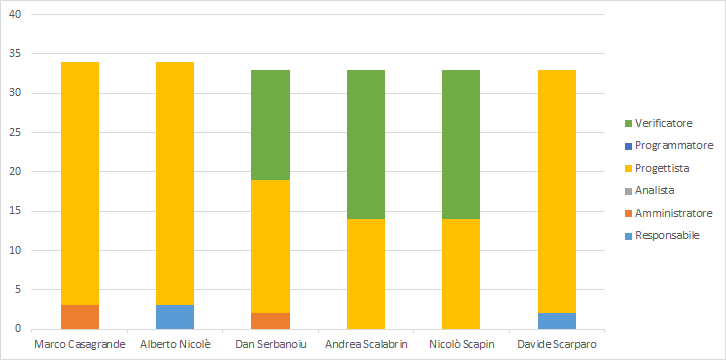
\includegraphics[scale=0.6]{img/6-2.png}
	\caption{Suddivisione ruoli per componente, Progettazione Architetturale}
\end{figure}

L'incidenza di tali ore determina in percentuale, come mostrato di seguito:
\begin{figure}[H]
	\centering
	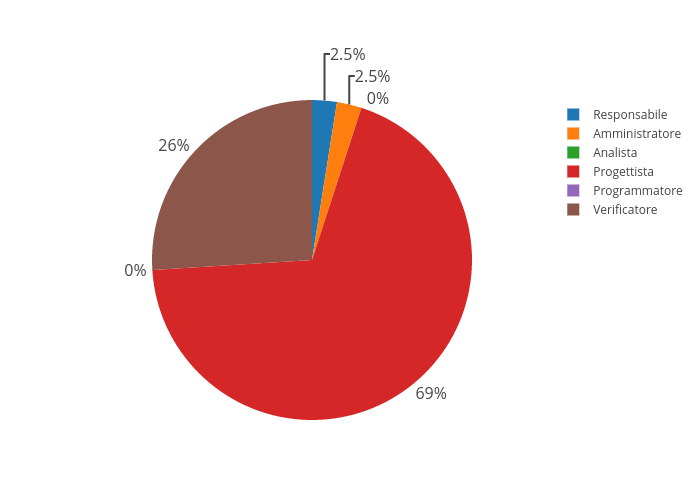
\includegraphics[scale=0.6]{img/ProgettazioneArchitetturale.png}
	\caption{Incidenza ore per ruolo, periodo di Progettazione Architetturale}
\end{figure}

\newpage
\subsection{Periodo di Progettazione Architetturale Dettagliata}
Il terzo periodo è la Progettazione Architetturale Dettagliata. Durante il corso di tale periodo, il lavoro dei membri sarà suddiviso come segue:

\begin{table}[H]
	\begin{center}
		\begin{tabular}{|c|c|c|c|c|c|c|c|}
			\hline
			\textbf{Nome} & \multicolumn{6}{c|}{\textbf{Ore per ruolo}} & \textbf{Ore totali} \\\cline{2-7}
			& \textbf{Resp} & \textbf{Amm} & \textbf{An} & \textbf{Proj} & \textbf{Prog} & \textbf{Ver} & \\
			\hline
			\MC			&	2	&		&		&	6	&		&	11	&	19	\\
			\hline
			\AN			&		&		&		&	8	&   	&	11	& 	19	\\
			\hline
			\DAN		&	3	&		&		&	17	&		&		&	20	\\
			\hline
			\AS			&		&	3	&	 	&	17	&	 	& 		&	20	\\
			\hline
			\NS 		&		&	3	&		&	17	&		& 		&	20	\\
			\hline
			\DS			& 		&		&		&	7	&		&	13	&	20	\\
			\hline
			\textbf{Totali per ruolo}	& 	5	&	6	&		&  72	&		&	35	&	118	\\
			\hline
		\end{tabular}
	\end{center}
	\caption{Ore per componente, Progettazione Architetturale Dettagliata}
\end{table}

\begin{figure}[H]
	\centering
	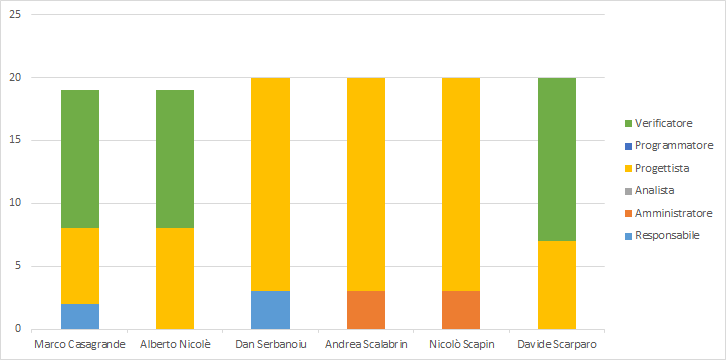
\includegraphics[scale=0.6]{img/6-3.png}
	\caption{Suddivisione ruoli per componente, Progettazione Architetturale Dettagliata}
\end{figure}

L'incidenza di tali ore determina in percentuale, come mostrato di seguito:
\begin{figure}[H]
	\centering
	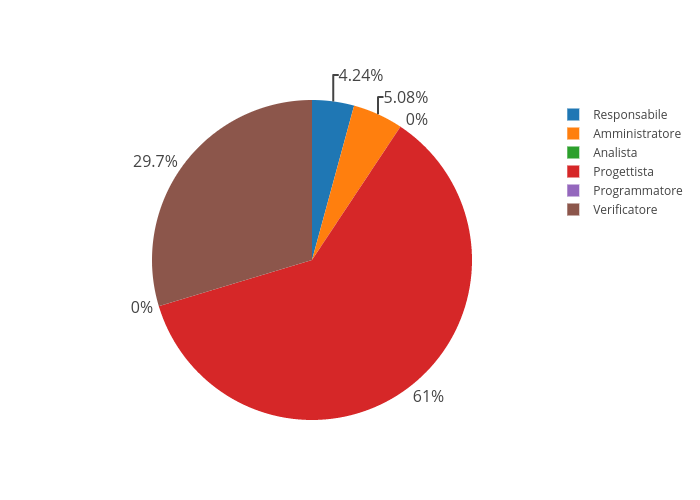
\includegraphics[scale=0.6]{img/ProgettazioneDettaglio.png}
	\caption{Incidenza ore per ruolo, periodo di Progettazione Architetturale Dettagliata}
\end{figure}

\newpage
\subsection{Periodo di Codifica}
Il penultimo periodo è la Codifica. Durante il periodo di Codifica, il lavoro dei membri sarà suddiviso come segue:

\begin{table}[H]
	\begin{center}
		\begin{tabular}{|c|c|c|c|c|c|c|c|}
			\hline
			\textbf{Nome} & \multicolumn{6}{c|}{\textbf{Ore per ruolo}} & \textbf{Ore totali} \\\cline{2-7}
			& \textbf{Resp} & \textbf{Amm} & \textbf{An} & \textbf{Proj} & \textbf{Prog} & \textbf{Ver} & \\
			\hline
			\MC			&		&		&		&		&	18	&	18	&	36	\\
			\hline
			\AN			&	3	&		&		&	 	&	32	&		& 	35	\\
			\hline
			\DAN		&		&		&		&		&	14	&	21	&	35	\\
			\hline
			\AS			&		&	 	&	 	&		&	14 	& 	22	&	36	\\
			\hline
			\NS 		&		&	3	&		&		&	32	& 		&	35	\\
			\hline
			\DS			& 	3	&		&		&		&	33	&		&	36	\\
			\hline
			\textbf{Totali per ruolo}	& 	6	&	3	&	143	& 	&		&	61	&	213	\\
			\hline
		\end{tabular}
	\end{center}
	\caption{Ore per componente, Codifica}
\end{table}

\begin{figure}[H]
	\centering
	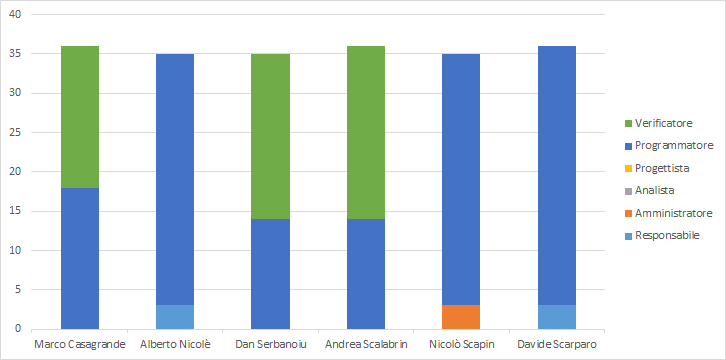
\includegraphics[scale=0.6]{img/6-4.png}
	\caption{Suddivisione ruoli per componente, Codifica}
\end{figure}

L'incidenza di tali ore determina in percentuale, come mostrato di seguito:
\begin{figure}[H]
	\centering
	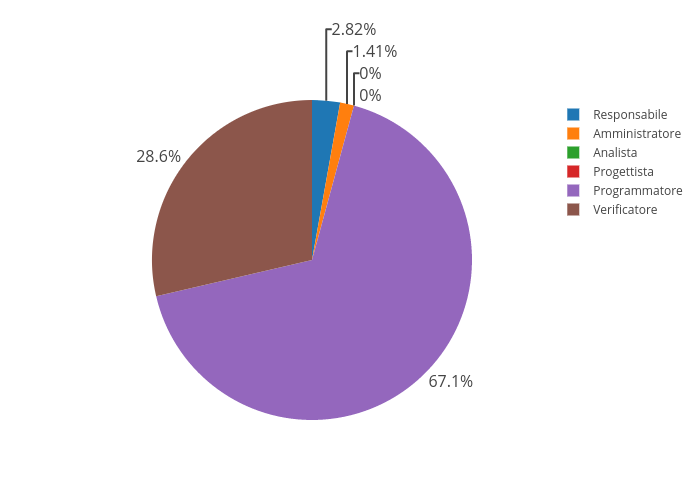
\includegraphics[scale=0.6]{img/Codifica.png}
	\caption{Incidenza ore per ruolo, periodo di Codifica}
\end{figure}

\newpage
\subsection{Periodo di Verifica e Validazione}
L'ultimo periodo è la Verifica e Validazione del prodotto sviluppato. Durante il periodo di Verifica e Validazione, il lavoro dei membri sarà suddiviso come segue:

\begin{table}[H]
	\begin{center}
		\begin{tabular}{|c|c|c|c|c|c|c|c|}
			\hline
			\textbf{Nome} & \multicolumn{6}{c|}{\textbf{Ore per ruolo}} & \textbf{Ore totali} \\\cline{2-7}
			& \textbf{Resp} & \textbf{Amm} & \textbf{An} & \textbf{Proj} & \textbf{Prog} & \textbf{Ver} & \\
			\hline
			\MC			&		&	3	&		&	7	&		&	6	&	16	\\
			\hline
			\AN			&		&		&		&	 	&		&	17	& 	17	\\
			\hline
			\DAN		&	3	&		&		&		&		&	14	&	17	\\
			\hline
			\AS			&		&	 	&	 	&	4	&	 	& 	12	&	16	\\
			\hline
			\NS 		&		&		&		&	4	&		& 	13	&	17	\\
			\hline
			\DS			& 		&		&		&		&		&	16	&	16	\\
			\hline
			\textbf{Totali per ruolo}	& 	3	&	3	&		&  15	&		&	78	&	99	\\
			\hline
		\end{tabular}
	\end{center}
	\caption{Ore per componente, Verifica}
\end{table}

\begin{figure}[H]
	\centering
	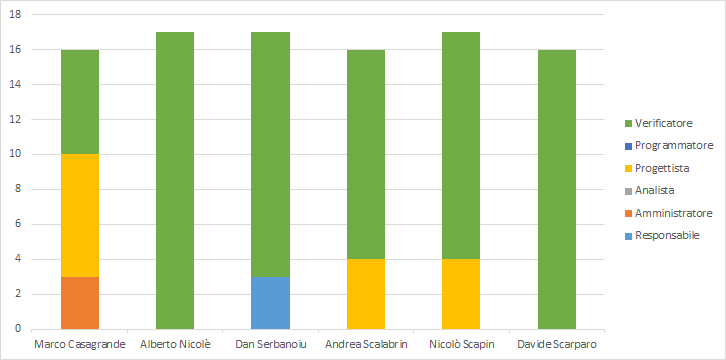
\includegraphics[scale=0.6]{img/6-5.png}
	\caption{Suddivisione ruoli per componente, Verifica}
\end{figure}

L'incidenza di tali ore determina in percentuale, come mostrato di seguito:
\begin{figure}[H]
	\centering
	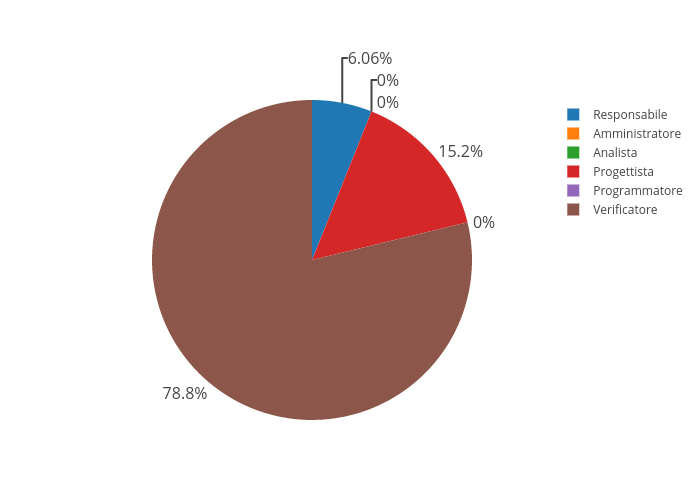
\includegraphics[scale=0.6]{img/Validazione.png}
	\caption{Suddivisione ore per ruolo, periodo di Verifica e Validazione}
\end{figure}

\newpage
\subsection{Ore di investimento}
La quota di investimento comprende le ore necessarie ad apprendere le tecnologie richieste per la realizzazione del progetto. Queste ore esulano dalle ore di \textit{Analisi dei Requisiti} e non sono a carico del \textit{Proponente}. L'investimento delle ore per auto formazione sulle tecnologie necessarie allo svolgimento del progetto si è concentrato principalmente nel periodo di progettazione, come mostrato di seguito.
\begin{figure}[H]
	\centering
	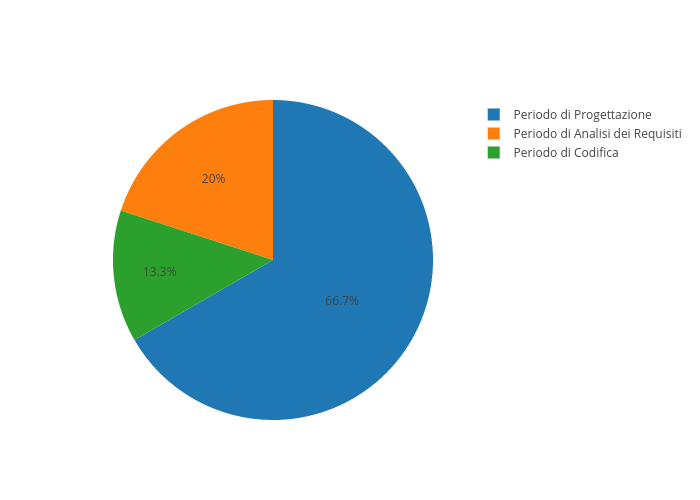
\includegraphics[scale=0.6]{img/ore_investimento_periodi}
	\caption{Ripartizione ore investimento}
	\label{fig:oreinvestimentoperiodi}
\end{figure}
Le ore complessive dedicate dai membri del gruppo sono 220 e riguardano auto formazione individuale sulle tecnologie necessarie e di indispensabile conoscenza da parte di tutti i membri del gruppo. Tutti i membri del gruppo, all'inizio del periodo di progettazione hanno affermato di avere buona padronanza delle seguenti tecnologie:
\begin{itemize}
	\item \textit{HTML5\ped{G}};
	\item \textit{CCS3\ped{G}};
	\item \textit{Java\ped{G}};
	\item \textit{MySQL\ped{G}}.
\end{itemize}
Le ore di auto formazione quindi, si sono concentrate sulle tecnologie rimanenti, ovvero:
\begin{itemize}
	\item \textit{Bootstrap 3\ped{G}};
	\item \textit{Jolie\ped{G}};
	\item \textit{JavaScript\ped{G}} e relativi framework:
	\begin{itemize}
		\item \textit{AngularJS\ped{G}};
		\item \textit{JQuery\ped{G}}.
	\end{itemize}
	\item \textit{Leonardo\ped{G}}.
\end{itemize}
Si segnala che un membro ha affermato di conoscere il framework \textit{Bootstrap 3}, per cui tralascerà l'auto formazione su tale tecnologia.

Di seguito sono riportate le ore che ogni membro ha dedicato all'auto formazione relativa alle tecnologie:

\begin{table}[H]
	\begin{center}
		\begin{tabular}{|c|c|}
			\hline
			\textbf{Ruolo}	& \textbf{Ore dedicate}  \\
			\hline
			\MC	&	33		\\
			\hline
			\DAN	&	34	\\
			\hline
			\AN	&	34		\\
			\hline
			\AS	&	31		\\
			\hline
			\NS	&	33		\\
			\hline
			\DS	&	32		\\
			\hline
			\textbf{Totale} & \textbf{197}  \\
			\hline
		\end{tabular}
	\end{center}
	\caption{Ore per auto formazione sulle tecnologie}
\end{table}


\subsection{Riepilogo}
Le ore totali del necessarie allo sviluppo sono 837 di cui, scorporando la fase di Analisi dei Requisiti, 630 remunerabili. Il consuntivo delle ore totali, raggruppate per ciascun membro del gruppo, e suddiviso per il ruolo assunto durante tutte le fasi del progetto, risulta essere così suddiviso:

\begin{table}[H]
	\begin{center}
		\begin{tabular}{|c|c|c|c|c|c|c|c|}
			\hline
			\textbf{Nome} & \multicolumn{6}{c|}{\textbf{Ore per ruolo}} & \textbf{Ore totali} \\\cline{2-7}
			& \textbf{Resp} & \textbf{Amm} & \textbf{An} & \textbf{Proj} & \textbf{Prog} & \textbf{Ver} & \\
			\hline
			\MC			&	2	&	7	&	16	&	44	&	18	&	52	&	139	\\
			\hline
			\AN			&	6	&	4	&	9	&	39	&	32	&	50	& 	139	\\
			\hline
			\DAN		&	6	&	4	&	32	&	34	&	14	&	49	&	139	\\
			\hline
			\AS			&	22	&	3 	&	12 	&	35	&	14 	& 	53	&	139	\\
			\hline
			\NS 		&	20	&	9	&	11	&	35	&	32	& 	32	&	139	\\
			\hline
			\DS			& 	5	&	2	&	5	&	38	&	33	&	57	&	139	\\
			\hline
			\textbf{Totali per ruolo}	& 	61	&	29	&	84	&  225	&	143	&	292	&	834	\\
			\hline
		\end{tabular}
	\end{center}
	\caption{Ore totali, per ruolo e componente}
\end{table}

La tabella sottostante, infine, raccoglie il conteggio complessivo delle ore remunerabili, suddivise per ruolo e componente.

\begin{table}[H]
	\begin{center}
		\begin{tabular}{|c|c|c|c|c|c|c|c|}
			\hline
			\textbf{Nome} & \multicolumn{6}{c|}{\textbf{Ore per ruolo}} & \textbf{Ore totali} \\\cline{2-7}
			& \textbf{Resp} & \textbf{Amm} & \textbf{An} & \textbf{Proj} & \textbf{Prog} & \textbf{Ver} & \\
			\hline
			\MC			&	2	&	6	&	0	&	44	&	18	&	35	&	105	\\
			\hline
			\AN			&	6	&	0	&	0	&	39	&	32	&	28	& 	105	\\
			\hline
			\DAN		&	6	&	2	&	0	&	34	&	14	&	49	&	105	\\
			\hline
			\AS			&	0	&	3 	&	0 	&	35	&	14 	& 	53	&	105	\\
			\hline
			\NS 		&	0	&	6	&	0	&	35	&	32	& 	32	&	105	\\
			\hline
			\DS			& 	5	&	0	&	0	&	38	&	33	&	29	&	105	\\
			\hline
			\textbf{Totali per ruolo}	& 	19	&	17	&	0	&  225	&	143	&	226	&	630	\\
			\hline
		\end{tabular}
	\end{center}
	\caption{Ore totali remunerabili, per ruolo e componente}
\end{table}

L'incidenza di tali ore incide in percentuale, come mostrato di seguito, prima complessive e poi remunerative:
\begin{figure}[H]
	\centering
	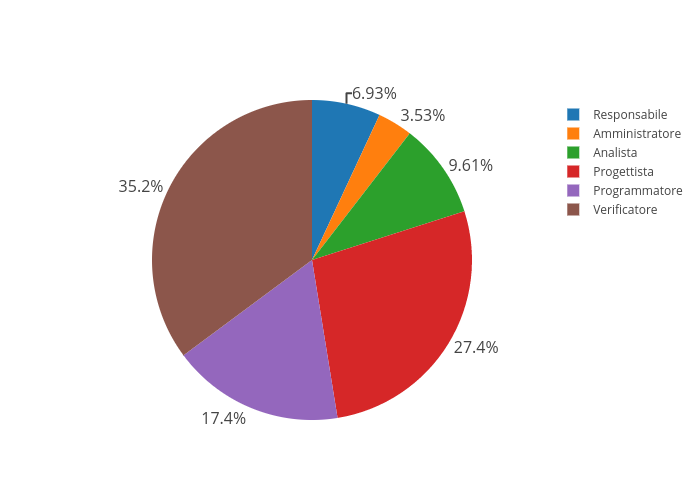
\includegraphics[scale=0.6]{img/OreTotali.png}
	\caption{Suddivisione ore per ruolo, riepilogo totale}
\end{figure}
\begin{figure}[H]
	\centering
	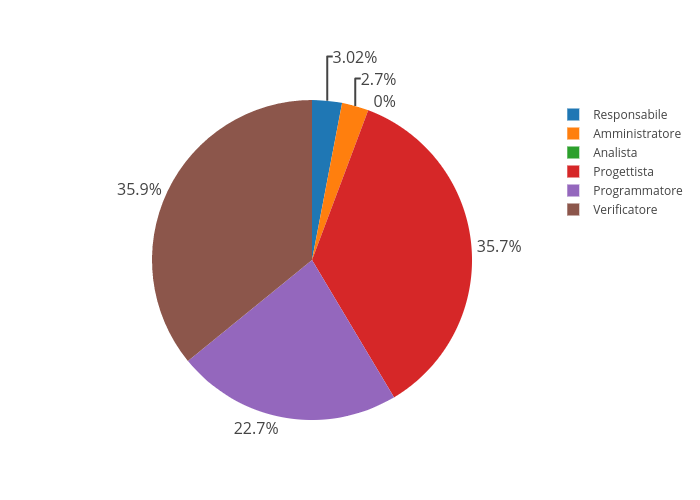
\includegraphics[scale=0.6]{img/OreRendicontabili.png}
	\caption{Suddivisione ore per ruolo, riepilogo ore remunerabili}
\end{figure}

